\documentclass{article}
\usepackage{authblk}
\usepackage[utf8]{inputenc}
\usepackage[T1]{fontenc}
\usepackage[ngerman]{babel}
\usepackage[normalem]{ulem}

\usepackage[pdftex]{graphicx}%package zum einbinden von Bildern
\usepackage{fancyhdr}
\usepackage{amsmath} %Paket für erweiterte math. Formeln
\usepackage{booktabs}%Weitere Optionen für Tabellen
\usepackage{array} 
\usepackage{float}
\usepackage{tabularx}
\usepackage[explicit]{titlesec}
\usepackage{color}
\usepackage{graphicx}
\usepackage[font=footnotesize]{caption} % define font-size for captions
\usepackage[font=footnotesize]{subcaption}
\usepackage{rotating}
\usepackage{longtable} 
\usepackage{dcolumn} 
\usepackage{pictex}
\usepackage{tikz} 

%============================================ Define Titlepage & packages =============================================%

\title{Notes 'Gewährleistung der Nachhaltigkeit in den Wäldern von RLP'}

\author{Andreas Hill}

\usepackage{fancyhdr}     
\usepackage{amsmath} %Paket für erweiterte math. Formeln
\usepackage[labelfont=bf]{caption}
\usepackage[font=footnotesize]{caption}
\usepackage[font=footnotesize]{subcaption}
\usepackage{graphicx}
\usepackage{caption}
\usepackage{subcaption}
\usepackage[final]{pdfpages}
\usepackage{color}

\usepackage{geometry}
\geometry{
	a4paper,
	left=25mm,
	right=25mm,
	top=30mm,
	bottom=30mm
}

\setlength{\parindent}{0em} % Einzug bei neuen Absätzen

%------------------------------------------------------------------------------------------------%
% -------------------------------------- Main Document------------------------------------------ %

\begin{document}

%------------------------------------------------------------------------------------------------%
% -------------------------------------- Tex Settings ------------------------------------------ %

\maketitle
\thispagestyle{empty}
\newpage

\pagenumbering{arabic}
\setcounter{page}{1}

\pagestyle{fancy} %Kopfzeile und Fusszeile
\fancyfoot[C]{\thepage}
\setlength{\headsep}{15mm}

\definecolor{mybrown}{rgb}{0.6, 0.15, 0.1}
\definecolor{amaranth}{rgb}{0.9, 0.17, 0.31}
\definecolor{mygreen}{rgb}{0.1, 0.4, 0.4}
\newcommand{\answer}[1]{\small \color{mybrown}{#1} \color{black}}
\newcommand{\note}[1]{\textit{\small \color{amaranth} \textbf{Note:} #1} \color{black}}
\newcommand{\todo}[1]{\color{red}{#1} \color{black}}
\newcommand{\answerfin}[1]{\small \color{mygreen}{#1} \color{black}}


%------------------------------------------------------------------------------------------------%
% ---------------------------------- Quelle 1 -------------------------------------------------- %

\section*{Richtlinie Nährstoffnachhaltigkeit 2017: Gewährleistung der Nährstoffnachhaltigkeit bei der Bewirtschaftung des Staatswaldes des Landes Rheinland-Pfalz}

% ++++++++++++++++++++++++++++++++++ %
\textbf{Zusammenfassung:}\\

\begin{itemize}
	
	\item Ziel: Gewährleistung der Nährstoffnachhaltigkeit
	
	\item Methode: Einteilung der Waldstandorte in sog. \textit{Vulnerabilitätsstufen} in Abhängigkeit von Standort (...) und Bestockung (...)
	
	\item Vulnerabilität drückt 'Verletzlichkeit des Waldökosystems gegenüber der Nicht-Einhaltung der Nährstoffnachhaltigkeit durch bspw. zu hohen Nährstoffentzugs im Zuge der Holzernte aus'.
	
	\item Darstellung der Vulnerabilitätstufen als Karte in Waldis. Soll als Grundlage bei der Hiebsplanung eingesetzt werden
	
	\begin{figure}[h]
		\centering
		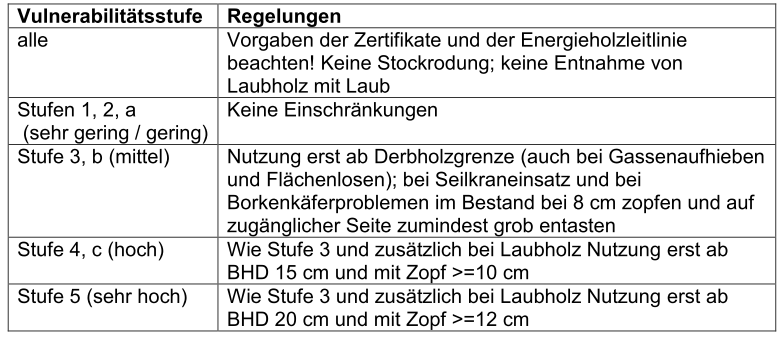
\includegraphics[scale=0.6]{Vulnerastufen.PNG}
		\caption{Vulnerabilitätsstufen}
		\label{fig:vulstufen}
	\end{figure}
	
	\item Es gibt \textbf{5 V-Stufen}. Bei allen Stufen sind die Vorgaben von Zertifikaten (FSC, PEFC, ...) zu beachten. Es ist zudem keine Stockrodung erlaubt (Ausnahme im Rahmen von Förderung). Zudem ist keine Entnahme von Laubholz im Laub gestattet.
		
\end{itemize} 
% ---------------------------------- %

% ++++++++++++++++++++++++++++++++++ %
\textbf{Hintergründe und Ziele:}\\

\begin{itemize}
	
	\item Trade-Off: Ausschöpfung des Nutzungspotentials (ökonom., Substitution fossiler Brennstoffe) vs. Nährstoffentzug (-> Nährstoffentzug ist ein wichtiger Aspekt des Nachhaltigkeitsziels)
	
	\item Ziel: Erhalt des \textit{Standortpotentials}, d.h \textit{Sicherung einer standortangepassten Versorgung}
	
	\item Richtlinie = Konzept zur Gewährleistung der Nährstoffnachhaltigkeit
	
	\item Methode: konkrete Angaben zur Anpassung der Nutzungsintensität je nach Standortpotential (Vuln.stufen).
	
	\item Grundlagen: waldortbezogene Bilanzierung und Schätzung der Bodenvorräte an Nährstoffen (Calcium, Magnesium, Kalium, Schwefel, Phosphor und Stickstoff) durch ein rechnergestütztes Decision Support System (\textit{DSS Nährstoffbilanzen}) -> Verweis auf Bericht "Endfassung Nährstoffbericht"
	
\end{itemize} 
% ---------------------------------- %


% ++++++++++++++++++++++++++++++++++ %
\textbf{Kurz: Nährstoffhaushalt von Waldökosystemen}\\

\begin{itemize}
	
	\item Nährstoffnachhaltigkeit: ausgeglichene oder positive Nährstoffbilanzen
	
	\item Bilanzierung: \textit{Eintrag} über atmosphärische Stoffdeposition u. Freisetzung von Nährstoffen aus Mineralverwitterung - \textit{Austrag} über Nährelementexport (via Holzernte und Sickerwasserausfluss)
	
	\item Einflussfaktoren \textit{Eintrag durch Niederschlag}: Abh. von Niederschlagshöhe (Deposition steigt mit Niederschlag) u. Bestockung (Fichte u. Douglasie zeigen höhere Depositionsraten als Kiefer, Buche und Eiche). 
	
	\item Nährst.freisetzung aus Mineralverwitterung ist abhängig vom Substrat und den klimatischen Bedingungen (Bodentemperatur, Bodenwassergehalt, Angriffsfläche des Gesteins) -> Parameter zusammengefasst in Substratreihe und Frischestufe.
	
	\item Einflussfaktoren \textit{Austrag durch Sickerwasser}: ... abh. von Substratreihe, Niederschlagsmenge und Bestockung (bei gleichen Bedingungen zeigen Fi und Dou höhere Austräge mit Sickerwasser als Kie, Buche u. Ei). 
	
	\item Einflussfaktoren \textit{Austrag durch Holzernte}: abh. von Standort, Baumart, Wuchsleistung, Nutzungsalter, Nutzungsintensität (Graphik in Präsi). 
	
	\item Kalium-Entzug bei Derbholznutzung (d.h. alles ab 7cm BHD): Buche >> Eiche > Fichte/Douglasie > Kiefer
	
	\item Magnesium-Entzug bei Derbholznutzung (d.h. alles ab 7cm BHD): Buche > Fichte > Eiche > Kiefer > Douglasie
	
	\item Höhe der Nährstoffentzüge steigen mit der Wuchsleistung
	
	\item Anteil der Nährstoffentzüge an Erntemasse ist in jungen Beständen deutlich höher als in älteren Beständen (höherer Rinden- und Reisiganteil).
	
	\item in Reife-Phase: 5-15\% der oberirdischen Biomasse entfallen auf die Rinde (!!! -> Überleitung zu Debarking Heads), ca. 10\% entfallen auf das Reisig (Def. reisig: Material < 7cm Durchmesser).
	
	\item Anteile bzgl. gespeicherter Nährstoffe: - bei Fichte und Douglasie ca. 50\% des oberird. Nährstoffvorrates im Reisig.
	
	\todo{Genauere Zahlen! Übersicht wäre schön.}
	
	\item Message O-Ton: \textit{'Daher ist die Entscheidung, welche Teile der 	Bäume genutzt werden und damit die Intensität der Nutzung, z.B. eine Beschränkung der Nutzung auf stofflich verwertbare höherwertige Sortimente (z. B. Stammholz), die Nutzung des gesamten Derbholzes (mit Rinde) oder die Nutzung der gesamten oberirdischen Biomasse (Vollbaumnutzung), von erheblichem Einfluss auf die Höhe der Entzüge an Biomasse und Nährstoffen.'}  
	
	\item Neben Bilanzen weitere Bewertungen: pflanzenverfügbare Vorräte im Boden für jeweilige Substratreihe in Abhängigkeit der Frischestufe geschätzt (über Frischestufe wird Feinbodenanteil geschätzt -> Feinbodenmenge beeinflusst Bodenvorräte). Schätzung Humusauflage durch Bestockungstyp (Phoshorvorrat in Humus: Kie > Fi > Dou > Bu > Ei) und Höhe ü. NN (Wärmeres Klima erhöht Bioturbation).

\end{itemize} 
% ---------------------------------- %

% ++++++++++++++++++++++++++++++++++ %
\textbf{Ausweisung der Vulnerabilitätsstufen}\\

\begin{itemize}
	
	\item Def. 'vulnerable': sensibel auf Störungen durch hohe Nutzungsintensität, es sind bei Nicht-Einhaltung der N-Richtlinie mit dauerhaften Einschränkungen wichtiger Funktionen wie bspw. einer Abnahme der Standortproduktivität zu rechnen
	
	\item 5 Stufen auf Basis der Indizes 'Nährstoffbilanz', Bodenvorrat, Nährstoffentzugsindex-Derbholnutzung u. Nährstoffentzugsindex-Vollbaumnutzung
	
	\item Stufe 1 (sehr geringe V.): feinbodenreiche Kalklehme des Devon, Magmatische Lehme aus Basalt
	
	\item Stufe 2 (geringe V.): Lößlehme / Schichtlehme des Rotliegenden
	
	\item Stufe 3 (mittlere V.): 
	
	\item Stufe 4 (hohe V.): tief basenarme Standorte aus Sanden des Buntsandsteins / Decklehme über Quarzit des Devon
	
	\item Stufe 5 (sehr hohe V.): tief basenarme Standorte aus Sanden des Buntsandsteins / Decklehme über Quarzit des Devon

\end{itemize} 
% ---------------------------------- %


% ++++++++++++++++++++++++++++++++++ %
\textbf{Vorgaben aus Zertifizierung PEFC, FSC u. Energieholzleitlinie}\\

\begin{itemize}
	
	\item PEFC: generell keine Ganzbaumnutzung (alle ober- und unterirdischen Baumteile). Vollbaumnutzung (alle oberirdischen Baumteile) nicht auf nährstoffarmen Böden, und auf nährstoffreichen Böden nicht häufiger als 2-4 mal im Bestandesleben (Ausnahme im Rahmen des Forstschutzes möglich). -> Vollbaumnutzung auf Stufe 1 und 2 Flächen eingeschränkt möglich.
	
	\item FSC: - alles unter Derbholzgrenze bleibt im Wald (Ausnahmen: Verkehrssicherung, Wegebau, Hochwasserschutz, Ersterschlissung/Gassenaufhiebe, Naturschutz, Weihnachtsbäume, Forstschutz - \todo{Vollbaumnutzung?}
	
	\item Energieholzleitlinie LForsten: - keine Nutzung von Kronenmaterial < 7cm Zopf mit Rinde (bei Laubholz < 10cm Zopf mit Rinde)

\end{itemize} 
% ---------------------------------- %


% ++++++++++++++++++++++++++++++++++ %
\textbf{Waldbaulischer Einfluss auf Nährstoffnachhaltigkeit}\\

\begin{itemize}
	
	\item Baumarten und Mischung -> wirkungsvollere Nutzung der Standortressourcen, Verbesserung der Standortsbedingungen. Erschliessung verfügbarer Nährstoffe in schlecht erschlossenen, dichten u. luftarmen Bodenbereichen durch tiefwurzelnde BAs (Weißtanne, Stiel- u. Traubeneiche), auf stauwasserfreien Standorten Douglasie.
	
	\item Verminderung des Risikos von Freilagen -> Auswaschungsverlusten entgegenwirken / Unterbrechung des Nährst-Kreislaufes vermeiden
	
	\item Aufgrund weitverbreiteter Stickstoffsättigung: Vermeiden einer Auswaschung von Nährstoffen durch beschleunigten Nährstofffreigabe von Nitrat, Kalium, Ca u. Mg. Daher Vermeiden von Bodenfreilagen und starker Konzentration von Hiebsresten.
	
	\item Waldbauliche Konsequenzen: stetiger, ununterbrochener Verbrauch der Nährstoffe durch 1) - frühzeitige Einleitung der Verjüngung.Flächendeckendes massives Aufkommen von Stickstoffweisern wie Brombeere, Brennessel, Weidenröschen und Springkraut sind Anzeichen für Stickstofffreisetzung und Auswaschung von Nährst.kationen.
	
	\item Bodenversauerung in Nadelwaldorten durch Einbringung von Laubbäumen abmildern

\end{itemize} 
% ---------------------------------- %


% ++++++++++++++++++++++++++++++++++ %
\textbf{Anpassung der Nutzungsintensität}\\

\begin{itemize}
	
	\item 



\end{itemize} 
% ---------------------------------- %


% ++++++++++++++++++++++++++++++++++ %
\textbf{Vorgaben}\\

\begin{itemize}
	
	\item keine Stockrodungen
	
	\item bei Laubbäumen keine Entnahme von Kronenmaterial
	
	\item Vollbaumnutzung nur bei V-Stufe 1 und 2 möglich und maximal bei jedem 2-ten Eingriff
	
	\item Additiv zur FSC-Regelung ist die Nutzung von Ncht-Derbholz bei Gassenaufhieben und Ersterschliessung bei V-Stufe 3, 4 u. 5 nicht zulässig. Dies gilt auch im Rahmen des Forstschutzes (auch bei Käferholz muss bei 8cm gezopft werden.)
	
	\item bei Harvestereinsätzen kommen keine Reisigmatten zum Einsatz, sonder statt dessen Buggibänder
	
	\item bei Seilkränen müssen die Bäume bei V-Stufe 3, 4, und 5 im Bestand gezopft und grob entastet werden
	
	\item bei V-Stufe 4 (5) sind Laubbäume mit BHD < 15cm (BHD < 20cm) am Fällort im Bestand zu belassen
	
	\item bei V-Stufe 4 (5) gilt bei Laubbäumen (\todo{was ist mit Nadelbäumen?}) ein Zopfdurchmesser von 10cm (12cm) mit Rinde
	
	
	
\end{itemize} 
% ---------------------------------- %


%------------------------------------------------------------------------------------------------%
\end{document}







